数学における格子は、何も難しい概念ではない。
特に、2次元の場合には視覚的にも分かりやすく、例えば、2つのベクトル
\begin{align*}
\mathbf{b}_1 = \begin{pmatrix}
1\\
2
\end{pmatrix},
\mathbf{b}_2 = \begin{pmatrix}
1\\
-1
\end{pmatrix}
\end{align*}
の整数結合$x_1\mathbf{b}_1 + x_2\mathbf{b}_2$の集合である。
図示するともっと分かりやすくて、$\mathbf{b}_1 + \mathbf{b}_2$や$2\mathbf{b}_1 - \mathbf{b}_2$、$-2\mathbf{b}_1 - 3\mathbf{b}_2$などという点が格子状に配置されている(\ref{fig:lattice_example})。

\begin{figure}[htb]
\begin{center}
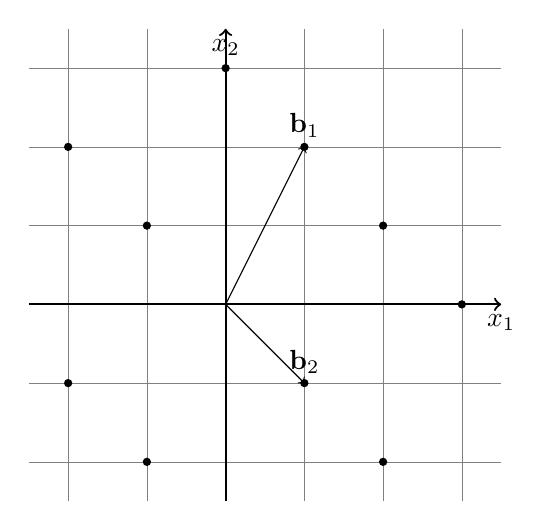
\begin{tikzpicture}
\draw [help lines] (-2.5,-2.5) grid (3.5,3.5);
\draw[thick, ->] (-2.5,0) -- (3.5,0) node [below] {$x_1$};
\draw[thick, ->] (0,-2.5) -- (0,3.5) node [below] {$x_2$};
\coordinate (O) at (0,0);
\coordinate (b1) at (1,2) node at (b1) [above] {$\mathbf{b}_1$};
\draw [->] (O) -- (b1);
\coordinate (b2) at (1,-1) node at (b2) [above] {$\mathbf{b}_2$};
\draw [->] (O) -- (b2);
\fill (b1) circle (1.5pt) (b2) circle (1.5pt) (2,1) circle (1.5pt) (0,3) circle (1.5pt) (2,-2) circle (1.5pt) (3,0) circle (1.5pt) (-1,1) circle (1.5pt) (-2,2) circle (1.5pt) (-1,-2) circle (1.5pt) (-2,-1) circle (1.5pt);
\end{tikzpicture}
\caption{$x_1\mathbf{b}_1 + x_2\mathbf{b}_2$の成す格子}
\label{fig:lattice_example}
\end{center}
\end{figure}

同じ点集合は、何も$\mathbf{b}_1,\mathbf{b}_2$でなくとも作れる。
例えば、$\mathbf{b}_1'=\begin{pmatrix}0\\3\end{pmatrix},\mathbf{b}_2' = \begin{pmatrix}1\\-1\end{pmatrix}$でも、$x_1\mathbf{b}_2' + x_2\mathbf{b}_2'$がまったく同じ点集合を成す。
実際、$\mathbf{b}_1'-\mathbf{b}_2'=\mathbf{b}_1$であることからも明らかだ。
同じようにして、どんな長いベクトルでも作れてしまうが、逆に「同じ点集合を表すベクトルの集合で、なるべく短いものは何か?」という疑問が生まれる。
それが最短ベクトル問題であり、暗号理論の分野ではしばしば暗号方式の安全性の根拠に使われる程難しい問題である。
一方で応用範囲はいくつもあり、例えばRSA暗号への攻撃手法の1つにも最短ベクトル問題が関係している\Notes{RSA暗号の秘密鍵$d$が小さいと破られることが知られている。なお、\textbf{RSA暗号が破られること}と\textbf{素因数分解ができること}は等価ではないので注意。}し、もちろん本稿の主題でもある素因数分解にも使える。

